\documentclass[12pt,a4paper]{article}
\usepackage[utf8]{inputenc}
\usepackage[T1]{fontenc}
\usepackage{amsmath}
\usepackage{amsfonts}
\usepackage{amssymb}
\usepackage{lipsum}
\usepackage{textcomp}

\usepackage{makecell} % linebreak dans une cellule
\usepackage{multicol} % twocols localement
\usepackage{vwcol} % idem mais avec largeur variable
\usepackage{color, colortbl} % colorer les tableaux
\usepackage{enumitem} % utiliser des lettres pour énumérer
\usepackage{wrapfig} % insérer des images dans dutexte
\usepackage{dashundergaps} % transformer du texte en ________
\usepackage{MnSymbol,wasysym} % smileys
\usepackage{ifthen}
\usepackage{soul} % teste barré \st

% --- geometry ---
\usepackage{geometry}
\geometry{legalpaper, margin=2cm}
% ---

% --- xcolor ---
\usepackage{xcolor}
\definecolor{lightgray}{gray}{0.9}
% ---

% --- tcolorboxes ---
\usepackage[most]{tcolorbox}
\newtcolorbox{definition}[2][]{%
  attach boxed title to top left
               = {yshift=-8pt},
  colback      = white,
  colframe     = gray,
  fonttitle    = \bfseries,
  colbacktitle = gray,
  title        = #2,#1,
  enhanced,
}
% ---


\renewcommand{\baselinestretch}{1.15} % augmenter l'interligne

\dashundergapssetup{
	teacher-gap-format=underline,
	gap-widen
}



\author{Paul Clavier}
\title{Chapitre 7 - Cercles et polygones réguliers}

\begin{document}

% --- Section & subsection renum ---
\renewcommand\thesection{\Roman{section}}
\renewcommand\thesubsection{\arabic{subsection}}
% ---

% --- Selection manuelle de la version ---
%\def\isprof{true}
% ---

% --- Selection automatique de la version ---
\ifdefined\isprof
	\TeacherModeOn
\fi

% ---



\begin{center}
	\fbox{\parbox{\dimexpr\linewidth-2\fboxsep-2\fboxrule\relax}{\centering\huge Chapitre 7 - Cercles et polygones réguliers\\Livre des ombres}}
\end{center}

\textit{Fais ta construction au crayon à papier.}

Étapes de construction:

\begin{enumerate}
\item Au milieu de la page, trace un triangle équilatéral ABC de côté 6 cm.
\item Place un point I milieu de [AB], un point J milieu de [AC] et un point K milieu de [CB].
\item Trace trois cercles de rayon 3 cm et de centre I, J et K.
\item Trace trois cercles de rayon 2,7 cm et de centre I, J et K.
\item Trace les segments [BJ], [AK] et [CI]. Place O le point d’intersection des segments.
\item Trace un cercle de centre O de rayon 2,5 cm puis un cercle de centre O de rayon 2,2 cm.
\item Repasse au feutre noir les demi-cercles situés vers l'intérieur du triangle ainsi que les cercles de centre O comme sur le dessin ci-dessous:
\begin{center}
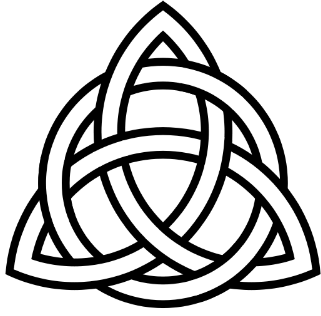
\includegraphics[scale=1]{img/Screenshot_2020-02-06 charmed_livre_des_ombres pdf.png}
\end{center}

\item Efface tes traits de construction et colorie ton dessin.

\end{enumerate}

\end{document}